\chapter{Summary and Conclusion}
\label{chapter: Conclusion}

The success or failure of a machine learning or deep learning process is directly proportional to the data quality used. The data source used in this work, the 2019 ISIC dataset, presented several problems that required the application of treatments to ensure the elimination of biases and the project's viability. For one, the data were collected from different medical sources at different resolutions. On the other hand, there was a very significant difference in the number of elements per class, resulting in a very unbalanced dataset. For the first case, the images were transformed to the resolution required by the neural networks. In the second case, two different strategies were used. The first consisted of trimming the samples according to the maximum number in the minority class. Although this technique is easy to apply, its disadvantage is the loss of the richness the discarded data could bring to the model's training. To compensate for this, we have opted for a second option: enriching the minority classes with synthetic images using SMOTE. This technique has allowed us to increase the total number of images processed from 250 per class to 300, an increase of 20%, and with both the first and second options, it has been possible to train the models with a balanced dataset. 

Transfer learning techniques were used to train the model. For this purpose, a classifier has been assembled using a feature extractor based on two well-known networks on the market, EfficientNet B0 and ResNet50, loaded with the weights from their training in ImageNet. This technique has allowed us to take advantage of the extractor's pattern recognition capabilities and complement it with a classifier stage. During the evolution of this work, the three steps of the transfer learning process have been demonstrated, showing that in the second step, a substantial improvement of the classification metrics of the network was already achieved.

The two assembled networks have been tested with the two treated datasets, the one that has been pruned and the one that has had the number of samples artificially increased employing SMOTE after that. As a result, we have seen that while the EfficientNet-based classifier does not show any significant difference between training with one or the other dataset, the ResNet50-based network improves its metrics when trained with the SMOTE-based dataset. One possible explanation for this process, as one network shows no improvement while the other does, can be found by comparing the depth of these networks. Indeed, if we examine the right-hand column of the table \ref{tbl: Metrics summary}, we can see a significant difference in the number of training parameters ResNet50 versus EfficienNet B0. Thus, a deeper network such as ResNet would benefit from training with a larger dataset.

\section{Metrics summary}

% Please add the following required packages to your document preamble:
% \usepackage{graphicx}
% \usepackage[table,xcdraw]{xcolor}
% Beamer presentation requires \usepackage{colortbl} instead of \usepackage[table,xcdraw]{xcolor}
\begin{table}[ht]
\centering
\resizebox{\textwidth}{!}{%
\begin{tabular}{l|cc|cc|cc|cc|cc|ccc}
\cline{2-11}
 & \multicolumn{2}{c|}{\cellcolor[HTML]{EFEFEF}\textbf{Acc}} & \multicolumn{2}{c|}{\cellcolor[HTML]{EFEFEF}\textbf{Sen}} & \multicolumn{2}{c|}{\cellcolor[HTML]{EFEFEF}\textbf{Esp}} & \multicolumn{2}{c|}{\cellcolor[HTML]{EFEFEF}\textbf{F1-score}} & \multicolumn{2}{c|}{\cellcolor[HTML]{EFEFEF}\textbf{Time (sec)}} & \multicolumn{1}{l}{} & \multicolumn{1}{l}{} & \multicolumn{1}{l}{} \\ \hline
\rowcolor[HTML]{EFEFEF} 
\multicolumn{1}{|l|}{\cellcolor[HTML]{EFEFEF}\textbf{Model name}} & \multicolumn{1}{c|}{\cellcolor[HTML]{EFEFEF}\textbf{\begin{tabular}[c]{@{}c@{}}No \\ SMOTE\end{tabular}}} & \textbf{\begin{tabular}[c]{@{}c@{}}With \\ SMOTE\end{tabular}} & \multicolumn{1}{c|}{\cellcolor[HTML]{EFEFEF}\textbf{\begin{tabular}[c]{@{}c@{}}No\\ SMOTE\end{tabular}}} & \textbf{\begin{tabular}[c]{@{}c@{}}With\\ SMOTE\end{tabular}} & \multicolumn{1}{c|}{\cellcolor[HTML]{EFEFEF}\textbf{\begin{tabular}[c]{@{}c@{}}No\\ SMOTE\end{tabular}}} & \textbf{\begin{tabular}[c]{@{}c@{}}With\\ SMOTE\end{tabular}} & \multicolumn{1}{c|}{\cellcolor[HTML]{EFEFEF}\textbf{\begin{tabular}[c]{@{}c@{}}No\\ SMOTE\end{tabular}}} & \textbf{\begin{tabular}[c]{@{}c@{}}With\\ SMOTE\end{tabular}} & \multicolumn{1}{c|}{\cellcolor[HTML]{EFEFEF}\textbf{\begin{tabular}[c]{@{}c@{}}No\\ SMOTE\end{tabular}}} & \textbf{\begin{tabular}[c]{@{}c@{}}With\\ SMOTE\end{tabular}} & \multicolumn{1}{c|}{\cellcolor[HTML]{EFEFEF}\textbf{\# Epochs}} & \multicolumn{1}{c|}{\cellcolor[HTML]{EFEFEF}\textbf{\begin{tabular}[c]{@{}c@{}}\# Trainable \\ params\end{tabular}}} & \multicolumn{1}{c|}{\cellcolor[HTML]{EFEFEF}\textbf{\begin{tabular}[c]{@{}c@{}}\# Total \\ params\end{tabular}}} \\ \hline
\multicolumn{1}{|l|}{\cellcolor[HTML]{EFEFEF}\textbf{model ENetB0 1}} & \multicolumn{1}{c|}{0.39} & 0.40 & \multicolumn{1}{c|}{0.40} & 0.45 & \multicolumn{1}{c|}{0.39} & 0.40 & \multicolumn{1}{c|}{0.38} & 0.39 & \multicolumn{1}{c|}{3191} & 3560 & \multicolumn{1}{c|}{40} & \multicolumn{1}{c|}{12808} & \multicolumn{1}{c|}{4064939} \\ \hline
\multicolumn{1}{|l|}{\cellcolor[HTML]{EFEFEF}\textbf{model ENetB0 2}} & \multicolumn{1}{c|}{0.45} & 0.40 & \multicolumn{1}{c|}{0.43} & 0.45 & \multicolumn{1}{c|}{0.44} & 0.40 & \multicolumn{1}{c|}{0.41} & 0.39 & \multicolumn{1}{c|}{2017} & 625 & \multicolumn{1}{c|}{8} & \multicolumn{1}{c|}{1361208} & \multicolumn{1}{c|}{4064939} \\ \hline
\multicolumn{1}{|l|}{\cellcolor[HTML]{EFEFEF}\textbf{model ENetB0 3}} & \multicolumn{1}{c|}{0.57} & 0.51 & \multicolumn{1}{c|}{0.59} & 0.54 & \multicolumn{1}{c|}{0.57} & 0.50 & \multicolumn{1}{c|}{0.55} & 0.49 & \multicolumn{1}{c|}{2925} & 3244 & \multicolumn{1}{c|}{40} & \multicolumn{1}{c|}{4020356} & \multicolumn{1}{c|}{4064939} \\ \hline
\multicolumn{1}{|l|}{\cellcolor[HTML]{EFEFEF}\textbf{model RNet1}} & \multicolumn{1}{c|}{0.27} & 0.31 & \multicolumn{1}{c|}{0.27} & 0.31 & \multicolumn{1}{c|}{0.27} & 0.31 & \multicolumn{1}{c|}{0.27} & 0.30 & \multicolumn{1}{c|}{2851} & 2266 & \multicolumn{1}{c|}{30} & \multicolumn{1}{c|}{20488} & \multicolumn{1}{c|}{23589384} \\ \hline
\multicolumn{1}{|l|}{\cellcolor[HTML]{EFEFEF}\textbf{model RNet2}} & \multicolumn{1}{c|}{0.80} & 0.83 & \multicolumn{1}{c|}{0.81} & 0.84 & \multicolumn{1}{c|}{0.80} & 0.82 & \multicolumn{1}{c|}{0.80} & 0.82 & \multicolumn{1}{c|}{179} & 210 & \multicolumn{1}{c|}{5} & \multicolumn{1}{c|}{15250440} & \multicolumn{1}{c|}{23589384} \\ \hline
\multicolumn{1}{|l|}{\cellcolor[HTML]{EFEFEF}\textbf{model RNet3}} & \multicolumn{1}{c|}{0.94} & 0.98 & \multicolumn{1}{c|}{0.94} & 0.98 & \multicolumn{1}{c|}{0.94} & 0.98 & \multicolumn{1}{c|}{0.94} & 0.97 & \multicolumn{1}{c|}{354} & 497 & \multicolumn{1}{c|}{8} & \multicolumn{1}{c|}{23539848} & \multicolumn{1}{c|}{23589384} \\ \hline
\end{tabular}%
}
    \caption{Table summarising metrics for each model}
    \label{tbl: Metrics summary}
\end{table}

The table \ref{tbl: Metrics summary} shows the values of the global metrics of the different training sessions. The first column on the left shows the name followed by a suffix indicating the step within the transfer learning process indicated in the section \ref{ch:Transfer_learning}. For each of the metrics, we find two columns that reflect the value obtained when the model has been trained with the balanced dataset after under-sampling (identified as "No SMOTE") and when the training has been performed with the dataset extended by over-sampling (identified as "With SMOTE"). In addition to the classical classification metrics, another column has been included with the training duration and the number of epochs. Calculating the quotient between both values allows us to extract the time per epoch, which can help make a training duration prediction by extending the number of epochs by the number of epochs. 

If we examine the accuracy and F1-score values of the first model, it can be empirically proven that it did not improve when trained with the SMOTE-enriched dataset. The opposite can be seen when observing the evolution of the values of the second network, with the important jump between the first and second steps, achieving good results in the third step. Let us compare the results obtained with both networks in the final step, the third. We see the significant difference between them, achieving with EfficientNet B0 in the best case, 57 \% accuracy, compared to 98 \% obtained by the ResNet50 network. Furthermore, with the third step, this model obtains very balanced metrics, both in sensitivity and specificity, translating into a high F1-score value, so we consider it an excellent multiclass classifier.

\section{Sample prediction}

\begin{figure}[ht]
    \centering
        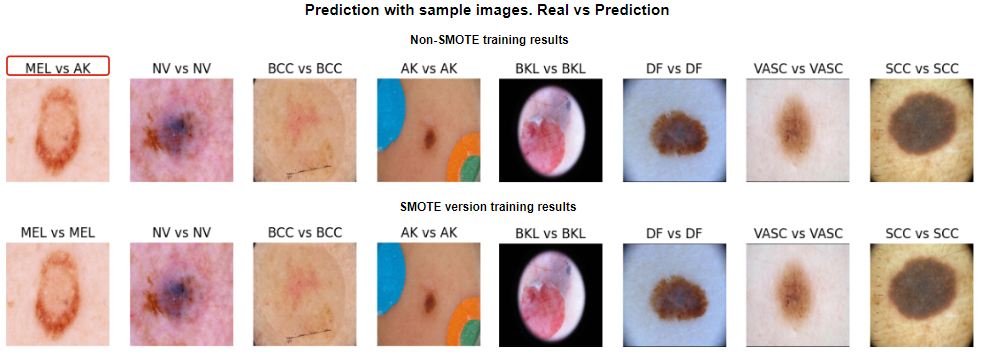
\includegraphics[scale=0.60]{images/Conclusion/Sample images Real vs Prediction.png}
        \caption{Test with a selection of sample images. Actual vs. Prediction Comparison}
    \label{fig: Sample Images real vs prediction}
\end{figure}

Finally, we have tested the predictive capacity of the ResNet50-based model, which obtained the best results in our study. In order to do so, one photograph from each class of the test dataset has been randomly selected from the test dataset. To follow the same line as the one used throughout our work, two models have been used: the model trained with the dataset that has been sup-sampled and the one that has been over-sampled with SMOTE. The results can be seen in the figure \ref{fig: Sample Images real vs prediction}. In the first line, we have the predictions obtained using the model trained with the first dataset, with a success rate of seven out of the eight samples (the wrong value has been marked). The second row shows the predictions obtained using the same model trained with the dataset treated with SMOTE, where the Convolutional network obtained a success of 100 \%

\section{Next steps}

To conclude this chapter, we would like to propose several lines of action to continue the work done:
\begin{itemize}
    \item The first of the most apparent actions is to increase further the level of synthetic samples performed with SMOTE. Considering that the minority class is above 200 samples, the hypothesis to prove or refute would be to see the maximum value of synthetic samples possible before the network stops learning due to the sample degradation for the feature repetition. In short, to find the ceiling of this over-sampling technique.
    \item The second item proposed is to perform tests with a deeper network than the ResNet 50. For example, a variant of the ResNet with 101 layers \cite{noauthor_resnet101_nodate} doubles the number of parameters to about 44 million. It is also possible to test the behavior using VGG16 \cite{simonyan_very_2015}, with approximately 138 million parameters, and even venture to test with a vision transformer (ViT) \cite{noauthor_papers_nodate}, an architecture different from the one used in this work, where attention mechanisms replace the convolutional layers. 
    \item Although we have seen that the capacity of the second network to classify is high, another point that could be worked on is the incorporation of filtering to eliminate or attenuate those undesired elements of the images, such as hairs or marks, to delimit the lesion.  
\end{itemize}



